\definecolor{exxetagray}{gray}{0.75}
\definecolor{itemcolor}{RGB}{179,217,255}
\definecolor{usercolor}{RGB}{255,204,179}

\shorthandoff{"}
\chapter{Ergebnisse}
\label{ch:ergebnisse}

\section{Ergebnisse der Mitarbeitendenbefragung}
An der Befragung der Mitarbeitenden bei EXXETA nahmen insgesamt 54 Mitarbeitende aus neun verschiedenen Teams teil.
Der Großteil der Befragten ($\approx$ 70 Prozent) stellten Mitarbeitende aus dem Team Java Enterprise Solutions dar, wobei sich die übrigen Mitarbeitenden nahezu gleichmäßg auf die anderen acht Teams (Business Application Development???) verteilt.
Die Befragung war für Mitarbeitende jedes Senioritätslevels und jeder Stellenbeschreibung zugängig.

% Von den 31 angefragten Fähigkeiten gaben Mitarbeitende im Mittel bei 38 Prozent der Fähigkeiten an Grundkenntnisse und bei 19 Prozent fortgeschrittene Kenntnisse zu besitzen (Werte aufgerundet auf die 2. Nachkommastelle).
% Bei knapp 43 Prozent der Fähigkeiten gaben die Befragten an, keine Kenntnisse zu besitzen.
% Von den angefragten Fähigkeiten wurden die Fähigkeiten "Backend" und "Git" von den meisten Mitarbeitenden beherrscht, während die Fähigkeit "Camunda" von den wenigsten Befragten besessen wurde.

% Von den angefragten Fähigkeiten wollten die befragten Mitarbeitenden im Durchschnitt 42 Prozent der Fähigkeiten in zukünftigen Projekten (weiter) anwenden.
% Bei 22 Prozent der Fähigkeiten gaben Mitarbeitende an, die Fähigkeit zukünftig (vorerst) nicht (weiter) anwenden zu wollen.
% Für 36 Prozent der Fähigkeiten gaben die Befragten an, der Möglichkeit, die Fähigkeit in zukünftigen Projekten anzuwenden, neutral gegenüber zu stehen.
% Übergreifend wurde die Fähigkeit "Git" von den meisten Mitarbeitenden präferiert, während die Fähigkeit "\ac{SOAP}" von den wenigsten Mitarbeitenden präferiert wurde.
% Der Fähigkeit "Helm" standen die meisten Mitarbeiter neutral gegenüber.
Insgesamt gaben die Befragten bei 960 der möglichen 1.674 Fähigkeiten (54 Probanden \`{a} 31 Fähigkeitsbewertungen) an, diese zu beherrschen, während sie bei den übrigen 714 Fähigkeiten angaben, keine Kenntnisse zu besitzen.
Von den beherrschten Fähigkeiten gaben die Mitarbeitenden bei zwei Drittel der Fähigkeiten an über Grundkenntnisse und bei den restlichen ein Drittel über fortgeschrittene Kenntnisse zu verfügen.
Bezüglich der Präferenzen gaben die Befragten bei einem Großteil (696 Bewertungen) der zu bewertenden Fähigkeiten an, diese zukünftig (weiter) in Projekten anwenden zu wollen.
Bei ähnlich vielen Fähigkeiten (607 Bewertungen) gaben die Mitarbeitende an, der Option, die Fähigkeit in zukünftigen Projekten anzuwenden, neutral gegenüberzustehen.
Lediglich bei rund einem Fünftel der bewerteten Fähigkeiten gaben die Befragten an, die Fähigkeit zukünftig (vorerst) nicht (weiter) anwenden zu wollen.

Die durchschnittliche Verteilung der Fähigkeiten und Präferenzen je Mitarbeitendem ist in Abbildung \ref{fig:ergebnisse:abb1} grafisch dargestellt.
Der blau hinterlegte Bereich stellt den Anteil der angefragten 31 Fähigkeiten dar, den ein Mitarbeitender im Mittel beherrscht (Anteile "Beherrscht und präferiert", "Beherrscht und neutral" und "Beherrscht, aber nicht präferiert").
Der gelb hinterlegte Bereich illustriert den Anteil der übrigen Fähigkeiten, den ein durchschnittlicher Mitarbeitender nicht beherrscht (Anteile "Nicht beherrscht, aber präferiert", "Nicht beherrscht und neutral" und "Nicht beherrscht und nicht präferiert").
% FARBEN ANPASSEN!

\begin{figure}
    \centering
	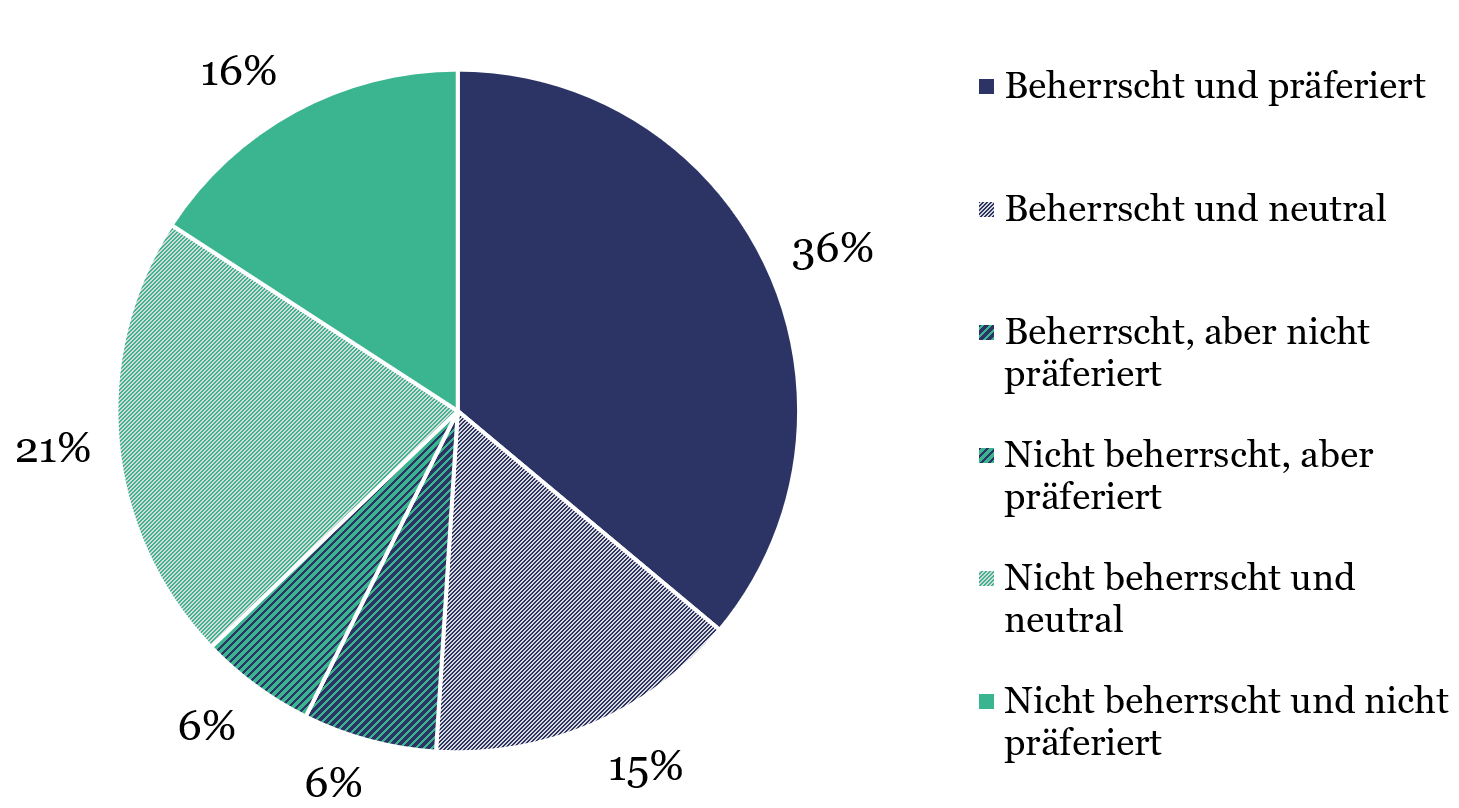
\includegraphics[width=1.0\textwidth]{gfx/verteilung-f-p.png}
	\caption[Durchschnittliche Verteilung der Fähigkeiten und Präferenzen je Mitarbeitenden]{Durchschnittliche Verteilung der Fähigkeiten und Präferenzen je Mitarbeitenden}
	\label{fig:ergebnisse:abb1}
\end{figure}

Aus dem Diagramm geht hervor, dass die Befragten im Durchschnitt mehr Fähigkeiten beherrschen (57 Prozent, blau hinterlegter Bereich), als nicht beherrschen (43 Prozent, gelb hinterlegter Bereich).
Mit 36 Prozent beherrscht und präferiert ein Mitarbeitender im Mittel den Großteil der insgesamt angefragten Fähigkeiten (blau markierter Bereich).
Von seinen beherrschten Fähigkeiten will ein Mitarbeitender folglich knapp zwei Drittel zukünftig weiter in Projekten einsetzen (36 von 57 Prozent).
Mit 21 Prozent treten bei einem durchschnittlichen Befragten am zweithäufigsten Fähigkeiten auf, in denen dieser keine Kenntnisse besitzt und indifferent ist, ob er diese Fähigkeiten zukünftig in Projekten anwenden wird, oder nicht (gelb hinterlegter Bereich mit grauen Punkten).
Darauf folgen 16 Prozent der angeforderten Fähigkeiten, die ein Mitarbeitender im Mittel nicht beherrscht und auch kein Interesse äußert, diese in zukünftigen Projekten anzuwenden (gelb markierter Bereich).
Weitere 15 Prozent der Fähigkeiten beherrscht ein durchschnittlicher Mitarbeitender und steht der Option, diese in zukünftigen Projekten einzusetzen, neutral gegenüber (blau hinterlegter Bereich mit grauen Punkten). 
Die übrigen 12 Prozent verteilen sich gleichmäßig auf die Fähigkeiten, die ein Mitarbeitender beherrscht, aber nicht präferiert (blau hinterlegter Bereich mit gelber Schraffur) und die Fähigkeiten, in denen ein Mitarbeitender keine Kenntnisse besitzt, diese aber präferiert (gelb hinterlegter Bereich mit blauer Schraffur).
Von den beherrschten Fähigkeiten haben Mitarbeitende im Mittel folglich bei circa 10 Prozent kein Interesse, diese beherrschten Fähigkeiten in Projekten (weiter) anzuwenden (6 von 57 Prozent).
Bei den nicht-beherrschten Fähigkeiten beläuft sich der Anteil an Fähigkeiten, die ein Mitarbeitender nicht beherrscht, aber zukünftig gerne in Projekten anwenden würde auf ganze 14 Prozent (6 von 43 Prozent).
% Demnach weist ein Mitarbeitender im Durchschnitt $2$ Fähigkeiten aus, die er nicht beherrscht, aber gerne anwenden würde und 2 Fähigkeiten die er beherrscht, aber kein Interesse hat, diese in Projekten weiter anzuwenden.

Die prozentuale Verteilung der Fähigkeiten und Präferenzen ist in Abbildung \ref{fig:ergebnisse:abb2} in Bezug auf die fünf Beispielprojekte dargestellt.

\begin{figure}
    \centering
	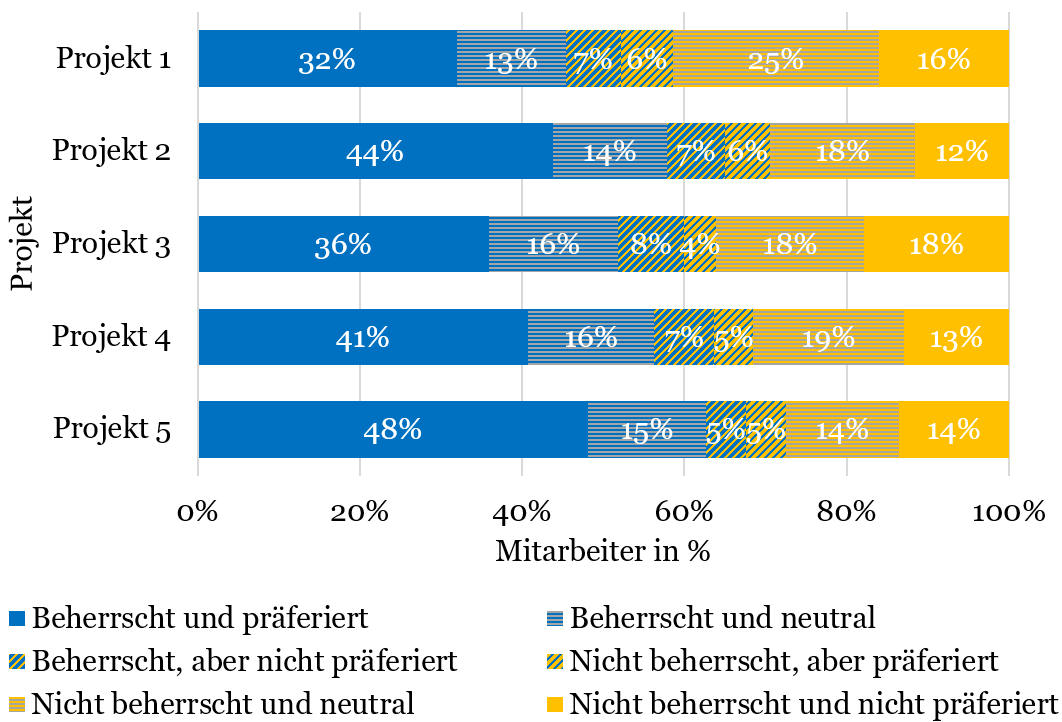
\includegraphics[width=0.95\textwidth]{gfx/verteilung-f-p-nach-projekt.png}
	\caption[Verteilung der Fähigkeiten und Präferenzen nach Projekt]{Verteilung der Fähigkeiten und Präferenzen nach Projekt}
	\label{fig:ergebnisse:abb2}
\end{figure}

Insgesamt wird deutlich, dass sich die Verteilung auf Projektebene nicht maßgeblich von der Ursprungsverteilung unterscheidet (Vgl. Abbildung \ref{fig:ergebnisse:abb1}).
Jedoch weist sie in einigen Punkten nennenswerte Abweichungen auf.
So geht aus der Abbildung hervor, dass Projekt 5 mit 48 Prozent die meisten Projektpositionen enthält, die Mitarbeitende als beherrscht und präferiert bewertet haben (blau markierter Balken).
Damit liegt die Verteilung der beherrschten und präferierten Fähigkeiten bei Projekt 5 um  12 Prozentpunkte über der Ursprungsverteilung.
Im Gegensatz dazu enthält Projekt 1 mit 32 Prozent die wenigsten Projektpositionen, die von den Befragten als beherrscht und präferiert angegeben wurden.
Diese Verteilung weicht jedoch lediglich um 4 Prozentpunkte von der Ursprungsverteilung ab.
Auch der Anteil der Projektpositionen, die Mitarbeitende nicht beherrschen und auch in zukünftigen Projekten nicht anwenden wollen ist in Projekt 1 mit 16 Prozent im Vergleich zu den anderen Projekten am zweithöchsten (gelb markierter Balken).
Lediglich Projekt 3 weist mit 18 Prozent mehr Projektpositionen auf, die Mitarbeitende nicht beherrschen und nicht präferieren.
Der Anteil an Projektpositionen, die Mitarbeitende nicht beherrschen und in denen sie der Option, diese zukünftig in Projekten anzuwenden neutral gegenüberstehen, ist dafür in Projekt 1 mit 25 Prozent am höchsten (gelb markierter Balken mit grauer Schraffierung).
Insgesamt weist Projekt 2 den nierdrigsten Anteil an Projektpositionen auf, die Mitarbeitende nicht beherrschen und nicht präferieren.
Dieser liegt mit 12 Prozent 4 Prozentpunkte unter der Ursprungsverteilung.
% Erklärungen für die schwankunen in den Verteilungen in Diskussion anführen -> Erklärung bspw., dass projekte untersch. viele fähigkeiten anfragen und teilweise sehr generisch und am bsp. von projekt 1 sehr spezifisch (bsp. Camunda, welches die fähigkeit ist, die am wenigsten MA beherrschen) (siehe oben auskommentierter text)
% Hier anführen, dass das darauf zurückzuführen sein kann, dass projekt 1 als einziges 12 fähigkeiten verlangt

\subsection{Zufriedenheit der Mitarbeitenden mit den Projektpositionen}
Hinsichtlich der Zufriedenheit gaben die Mitarbeitenden mit 146 von insgesamt 270 Bewertungen (54 Probanden \`{a} 5 Beispielprojekte) bei mehr als der Hälfte der Optionen an, mit einem Beispielprojekt nicht zufrieden zu sein (Anteile "Gar nicht zufrieden" und "Weniger zufrieden").
Darüber hinaus wurde die Bewertung "Voll und ganz zufrieden" mit 43 Bewertungen am wenigsten von den Befragten angegeben.
Am häufigsten gaben die Mitarbeitenden an mit einem Beispielprojekt gar nicht zufrieden zu sein (83 Bewertungen).

In Abbildung \ref{fig:ergebnisse:abb3} ist die Zufriedenheit der Mitarbeitenden anhand der einzelnen Projekte abgebildet.
Daraus geht hervor, dass die Mitarbeitenden mit insgesamt 55 Prozent am häufigsten angaben mit Projekt 4 zufrieden zu sein (Anteile "Eher zufrieden" und "Voll und ganz zufrieden").
Mit Projekt 3 waren die Befragten im Vergleich am wenigsten zufrieden.
Der Anteil der zufriedenen Mitarbeitenden lag hier bei 31 Prozent.
Verglichen mit der Verteilung der Fähigkeiten und Präferenzen in Abbildung \ref{fig:ergebnisse:abb2} fällt auf, dass bei Projekt 3 auch der Anteil der Fähigkeiten, die von den Mitarbeitenden nicht präferiert wurden mit 26 Prozent am höchsten ausfiel (blau hinterlegter Balken mit gelber Schraffur und gelb markierter Balken).

\begin{figure}[H]
    \centering
	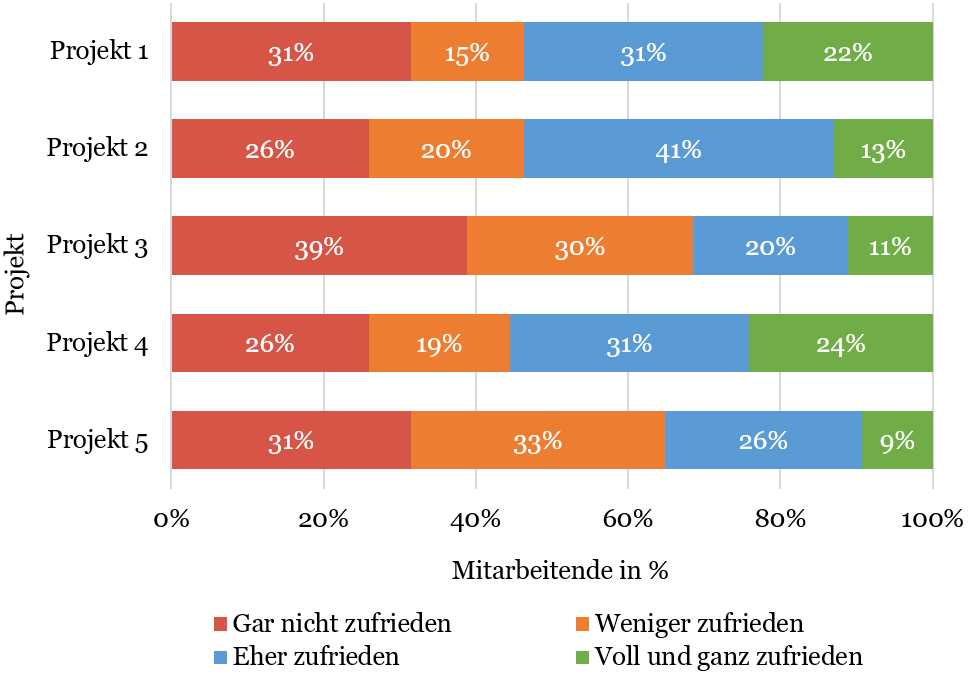
\includegraphics[width=0.95\textwidth]{gfx/verteilung-z-nach-projekt.png}
	\caption[Zufriedenheit der Mitarbeitenden nach Projekt]{Zufriedenheit der Mitarbeitenden nach Projekt}
	\label{fig:ergebnisse:abb3}
\end{figure}

\subsection{Angegebene Zufriedenheit vs. Präferenzangaben}
Im Zusammenhang mit der angegebenen Zufriedenheit der Mitarbeitenden wurde außerdem untersucht, wie sehr die angegebenen Präferenzen der Mitarbeitenden mit den angeforderten Projektpositionen übereinstimmen.
Abbildung \ref{fig:ergebnisse:abb4} zeigt die Verteilung der Mitarbeitenden anhand der Rate der Übereinstimmung ihrer Präferenzen mit den angeforderten Projektpositionen nach Projekt.
Ein Histogramm bildet je Intervall die Anzahl der Mitarbeitenden ab, deren Rate der Übereinstimmung in das jeweilige Intervall fällt.

\begin{figure}[H]
    \centering
    \subfloat[Projekt 1]{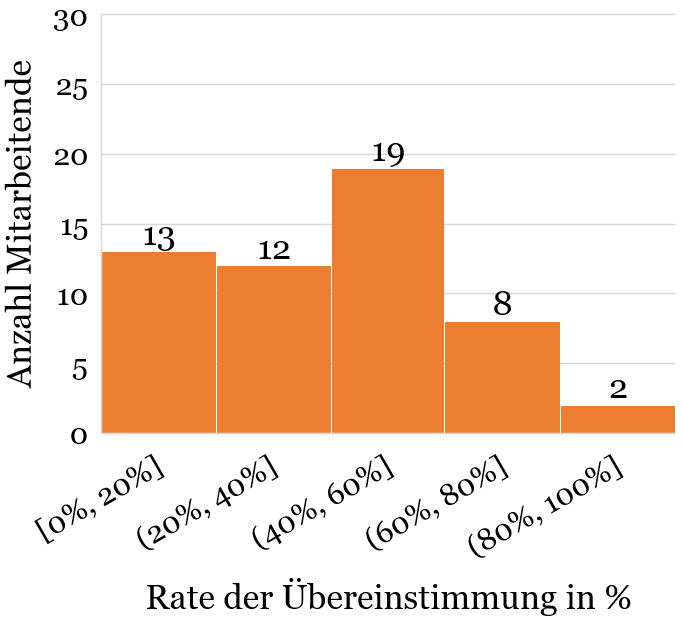
\includegraphics[width=0.5\textwidth]{gfx/verteilung-p-z-hist-p1.png}\label{fig:ergebnisse:abb4:1}}
    \subfloat[Projekt 2]{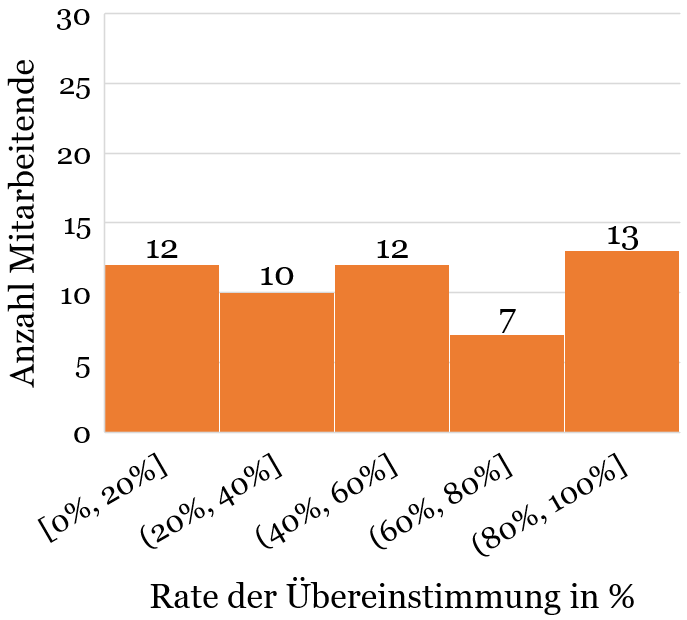
\includegraphics[width=0.5\textwidth]{gfx/verteilung-p-z-hist-p2.png}\label{fig:ergebnisse:abb4:2}}\\
    \subfloat[Projekt 3]{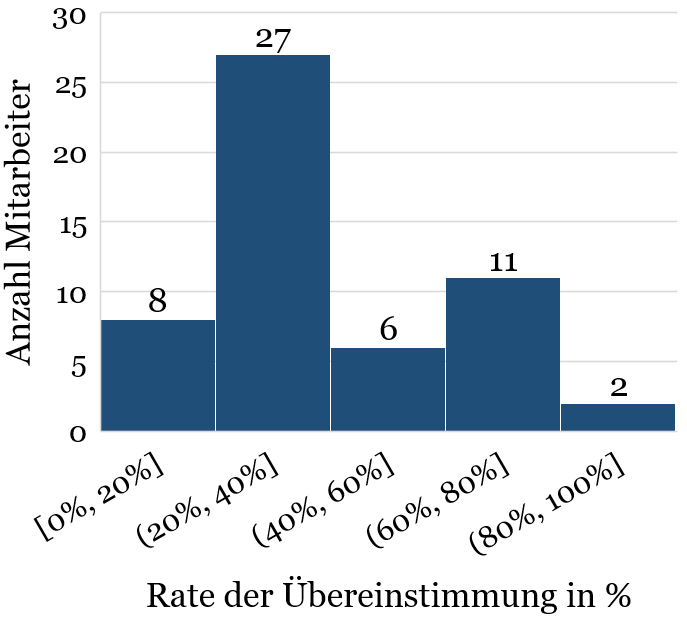
\includegraphics[width=0.5\textwidth]{gfx/verteilung-p-z-hist-p3.png}\label{fig:ergebnisse:abb4:3}}
    \subfloat[Projekt 4]{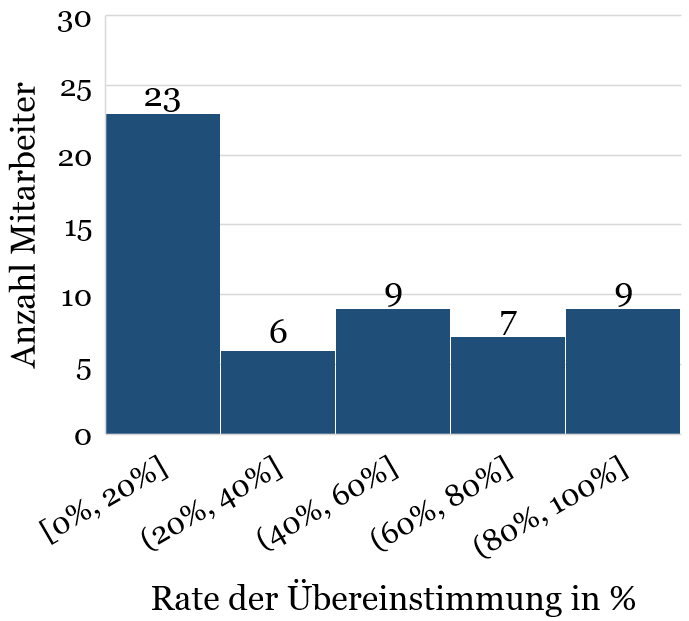
\includegraphics[width=0.5\textwidth]{gfx/verteilung-p-z-hist-p4.png}\label{fig:ergebnisse:abb4:4}}\\
    \subfloat[Projekt 5]{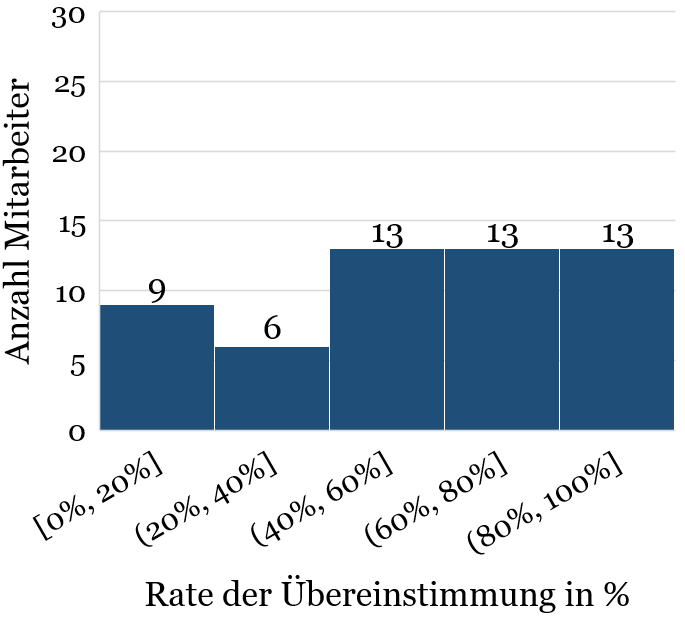
\includegraphics[width=0.5\textwidth]{gfx/verteilung-p-z-hist-p5.png}\label{fig:ergebnisse:abb4:5}}\\
\caption[Übereinstimmung der Präferenzen der Mitarbeitenden und angeforderten Projektpositionen nach Projekt]{Übereinstimmung der Präferenzen der Mitarbeitenden und angeforderten Projektpositionen nach Projekt}
  \label{fig:ergebnisse:abb4}
\end{figure}
Den Verteilungen ist zu entnehmen, dass die höchsten Übereinstimmung der Präferenzen der Mitarbeitenden mit den Projektpositionen bei Projekt 2 und Projekt 5 erreicht wurden.
Die Anzahl der Befragten, die eine Übereinstimmung über 80 Prozent erreichten lag hier je Projekt bei 13 Mitarbeitenden.
Insgesamt ist die Anzahl der Mitarbeitenden, die eine mittlere bis hohe Übereinstimmung aufwiesen (Rate der Übereinstimmung größer 40 Prozent) bei Projekt 5 mit 39 Befragten am höchsten.

Auffällig ist, dass trotz der hohen Übereinstimmung der Präferenzen mit den angeforderten Projektpositionen von Projekt 5, bei der Befragung der Zufriedenheit lediglich 35 Prozent der Befragten angaben mit dem Projekt 5 zufrieden zu sein (Vgl. Abbildung \ref{fig:ergebnisse:abb3}).
Im Verhältnis zu den anderen Projekten ist Projekt 5 hinsichtlich der angegebenen Zufriedenheit der Mitarbeitenden damit das Projekt mit der zweitkleinsten Anzahl zufriedener Befragter.
% den kommenden teil in die diskussion packen?
Ein detaillierter Abgleich der Mitarbeitenden, die angaben mit Projekt 5 zufrieden zu sein, mit den Mitarbeitenden, die eine hohe Übereinstimmung aufwiesen (> 80 Prozent) zeigte, dass lediglich 5 dieser 13 Mitarbeitenden auch angaben, mit dem Projekt zufrieden zu sein.
Weiter ist zu erkennen, dass Projekt 4 zwar bei der Befragung der Zufriedenheit die höchste Anzahl an zufriedenen Mitarbeitenden aufwies ($\approx$ 30 Befragte), in der Übereinstimmung der Präferenzen jedoch im Vergleich am zweitwenigsten Mitarbeitende eine Übereinstimmung über 40 Prozent aufwiesen.
Darüber hinaus liegt die Anzahl an Mitarbeitenden mit einer Übereinstimmung der Präferenzen unter 20 Prozent\footnote{inkl.} bei Projekt 4 mit 23 Befragten mit Abstand am höchsten.
% Hier wieder bei diskussion die  schwankung erklären -> annahme, dass das mit der ANzahl der angeforderten Projektpositionen zusammenhängt!

\section{Ergebnisse der Managerbefragung}
An der Befragung der Manager haben insgesamt vier Manager des Teams Java Enterprise Solutions teilgenommen.
Im Durchschnitt gab jeder Manager je Projekt 7 Mitarbeitende an, wobei individuell hohe Schwankungen zwischen den Anzahlen der Mitarbeitenden zu erkennen waren.
So gab der Manager, der projektübergreifend die meisten Mitarbeitenden nannte, insgesamt 66 Mitarbeitende an, während der Manager, der projektübergreifend die wenigsten Mitarbeitenden nannte, insgesamt nur 15 Mitarbeitende angab.

\subsection{Erwartete Arbeitsleistung der Mitarbeitenden nach Projekten}
In Abbildung \ref{fig:ergebnisse:abb5} ist die Anzahl der Mitarbeitenden mit zu erwartend hoher Arbeitsleistung je Projekt dargestellt.
Neben der Anzahl der Mitarbeitenden mit zu erwartend hoher Arbeitsleistung ist in dem Diagramm zusätzlich die Anzahl der Mitarbeitenden nach Reduktion der mehrfach genannten Mitarbeitenden (d.h. ohne Duplikate) abgetragen.

\begin{figure}
    \centering
	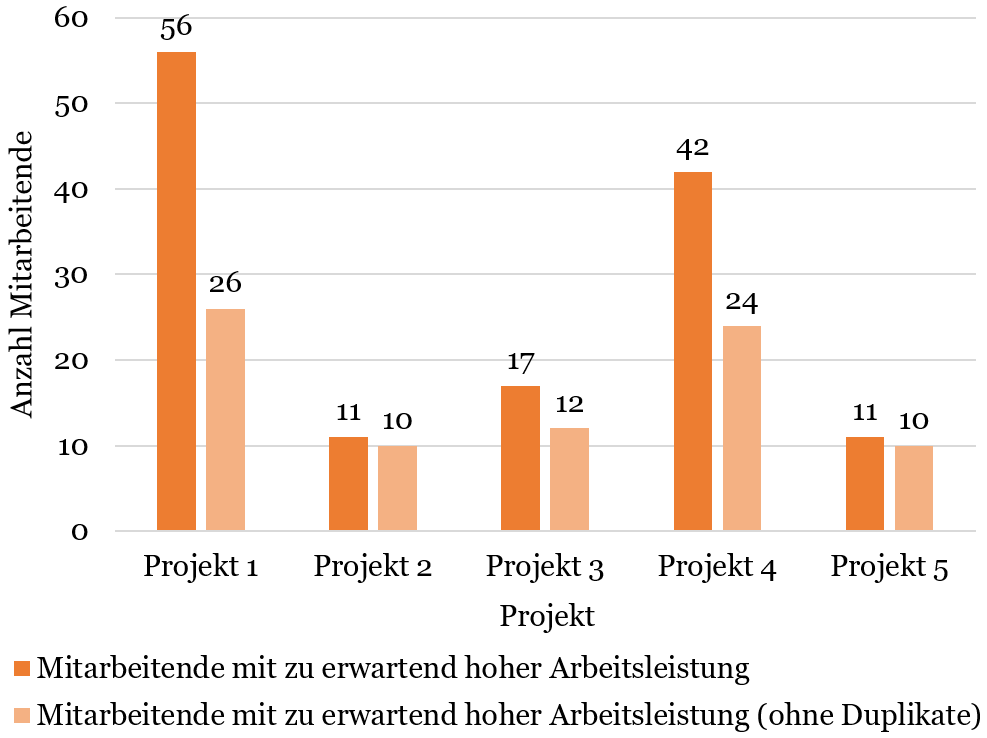
\includegraphics[width=0.9\textwidth]{gfx/verteilung-m-prod.png}
	\caption[Mitarbeitende mit zu erwartender hoher Arbeitsleistung nach Projekt]{Mitarbeitende mit zu erwartender hoher Arbeitsleistung nach Projekt}
	\label{fig:ergebnisse:abb5}
\end{figure}

Aus Abbildung \ref{fig:ergebnisse:abb5} geht hervor, dass die Befragten projektübergreifend mit 56 Angaben bei Projekt 1 am meisten Mitarbeitende angaben (dunkelblauer Balken).
Die Anzahl nach Entfernung der mehrfach genannten Mitarbeitenden reduziert sich bei Projekt 1 auf weniger als die Hälfte (26 Mitarbeitende, hellblauer Balken).
Eine solche Diskrepanz zwischen der Anzahl an genannten Mitarbeitenden und der Anzahl der Mitarbeitenden ohne Duplikate weist darauf hin, dass die einzelnen Manager in dem betroffenen Projekt überwiegend diesselben Mitarbeitenden ausgewählt haben.
Eine ähnlich hohe Diskrepanz ist bei den Angaben der Manager für Projekt 4 zu erkennen.
Insgesamt erwarteten die Manager bei Projekt 1 mit 26 genannten unterschiedlichen Mitarbeitenden die meisten Mitarbeitenden mit einer hohen Arbeitsleistung.
Die wenigsten Mitarbeitenden mit zu erwartend hoher Arbeitsleistung nannten die Manager bei Projekt 2 mit 9 erwarteten unterschiedliche Mitarbeitenden, eng gefolgt von Projekt 5 mit 10 erwarteten unterschiedlichen Mitarbeitenden.

\subsection{Erwartete Arbeitsleistung vs. Fähigkeitsangaben der Mitarbeitenden}
Hinsichtlich der zu erwartenden Arbeitsleistung der Mitarbeitenden wurde des Weiteren betrachtet, wie sehr die angegebenen Fähigkeiten der Mitarbeitenden aus der Mitarbeiterbefragung mit den angeforderten Projektpositionen übereinstimmen.
Die Verteilung der Mitarbeitenden anhand der Rate der Übereinstimmung ihrer Präferenzen mit den angeforderten Projektpositionen ist in Abbildung \ref{fig:ergebnisse:abb7} je Projekt dargestellt.
Analog zu den Histogrammen aus Abbildung \ref{fig:ergebnisse:abb4}, bildet jedes Histogramm je Intervall die Anzahl der Mitarbeitenden ab, deren Rate der Übereinstimmung in das jeweilige Intervall fällt.

\begin{figure}
    \centering
    \subfloat[Projekt 1]{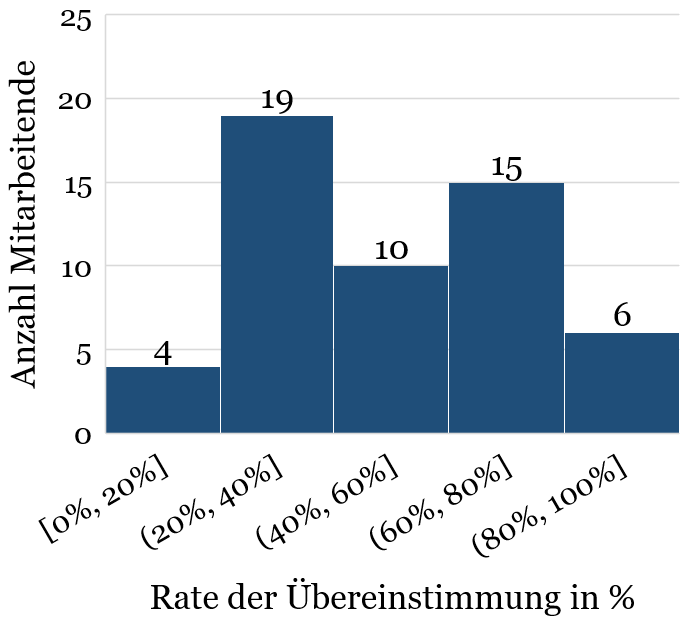
\includegraphics[width=0.5\textwidth]{gfx/verteilung-f-p-hist-p1.png}\label{fig:ergebnisse:abb7:1}}
    \subfloat[Projekt 2]{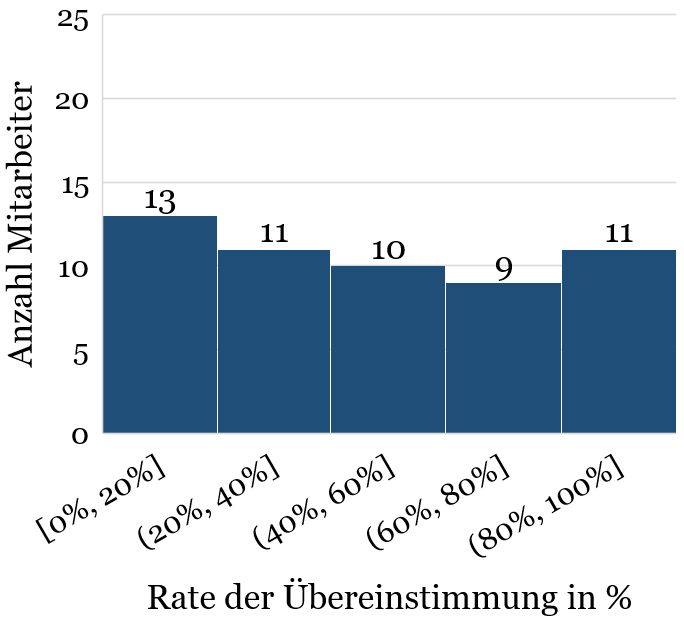
\includegraphics[width=0.5\textwidth]{gfx/verteilung-f-p-hist-p2.png}\label{fig:ergebnisse:abb7:2}}\\
    \subfloat[Projekt 3]{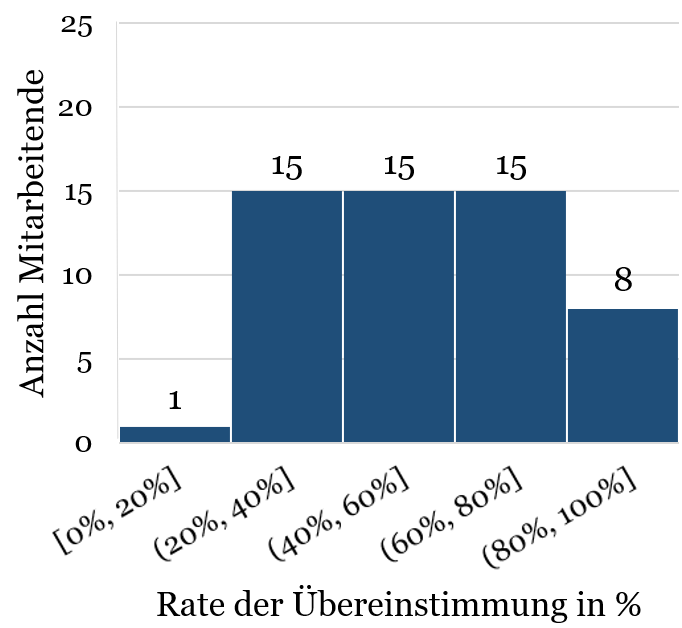
\includegraphics[width=0.5\textwidth]{gfx/verteilung-f-p-hist-p3.png}\label{fig:ergebnisse:abb7:3}}
    \subfloat[Projekt 4]{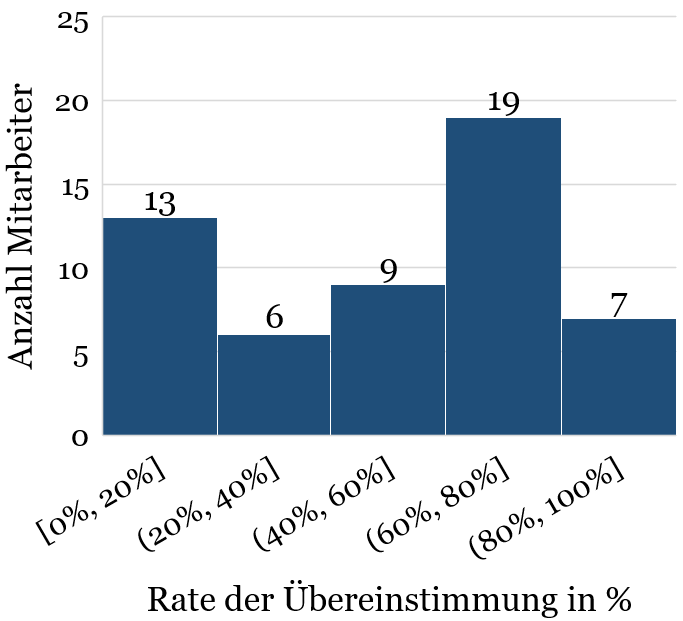
\includegraphics[width=0.5\textwidth]{gfx/verteilung-f-p-hist-p4.png}\label{fig:ergebnisse:abb7:4}}\\
    \subfloat[Projekt 5]{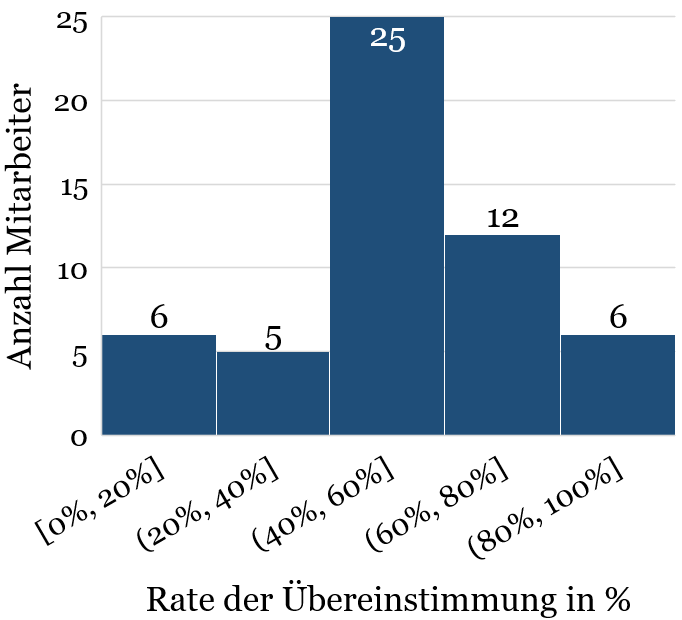
\includegraphics[width=0.5\textwidth]{gfx/verteilung-f-p-hist-p5.png}\label{fig:ergebnisse:abb7:5}}\\
\caption[Übereinstimmung der Fähigkeiten eines Mitarbeitenden mit den angeforderten Projektpositionen nach Projekt]{Übereinstimmung der Fähigkeiten eines Mitarbeitenden mit den angeforderten Projektpositionen nach Projekt}
  \label{fig:ergebnisse:abb7}
\end{figure}

Ein Vergleich der histografischen Verteilungen je Projekt in Abbildung \ref{fig:ergebnisse:abb7} zeigt, dass die größte Übereinstimmung ($>$ 80 Prozent) bei Projekt 2 vorliegt (Vgl. Abbildung \ref{fig:ergebnisse:abb7:2}).
Insgesamt wiesen 11 der 54 Mitarbeitenden eine hohe Übereinstimmung mit den Projektpositionen von Projekt 2 auf.
Verglichen mit der durch die Manager angegebenen erwarteten Arbeitsleistung aus Abbildung \ref{fig:ergebnisse:abb5} fällt auf, dass sich die Anzahl der Mitarbeitenden mit hoher Arbeitsleistung in einem ähnlichen Bereich befindet.
Für Projekt 2 gaben die Manager hier insgesamt 9 unterschiedliche Mitarbeitende an, von denen sie eine hohe Arbeitsleistung erwarten würden.
Ein Abgleich der Angabe der 9 Mitarbeitenden durch die Manager mit den 11 Mitarbeitenden mit der höchsten Übereinstimmung zeigte jedoch, dass lediglich 5 der 11 Mitarbeitenden mit höchster Übereinstimmung in der Auswahl der Mitarbeitenden durch die Manager vorkamen.

Weiter fällt auf, dass Projekt 2 die größte Anzahl an Mitarbeitenden aufweist, deren Fähigkeiten weniger als 40 Prozent\footnote{inkl.} mit den angeforderten Projektpositionen übereinstimmen.
Gemeinsam mit Projekt 4 weisen die Projekte mit je 13 Mitarbeitenden die meisten Mitarbeitenden auf, deren Übereinstimmung unter 20 Prozent\footnote{inkl.} fällt.
Konträr zu Projekt 2 besitzt Projekt 4 jedoch zugleich die größte Anzahl an Mitarbeitenden mit einer Übereinstimmung von Fähigkeiten mit Projektpositionen über 60 Prozent (Vgl. Abbildung \ref{fig:ergebnisse:abb7:4}).
Ein Abgleich der Angabe der 23 Mitarbeitenden durch die Manager mit den 26 Mitarbeitenden mit einer Übereinstimmung über 60 Prozent zeigte in diesem Fall, dass 22 der 23 fähgisten Mitarbeitenden mit den angegebenen Mitarbeitenden durch die Manager übereinstimmen.

% Abbildung \ref{fig:ergebnisse:abb6} stellt die mittlere Übereinstimmung der Fähigkeiten der Mitarbeitenden mit den angeforderten Projektpositionen je Projekt dar.
% In dem Diagramm ist die durchschnittliche Übereinstimmung der Fähigkeiten eines Mitarbeitenden mit den angeforderten Projektpositionen als Liniendiagramm dargestellt.
% Die Standardabweichung vom Mittelwert ist als Balkendiagramm abgebildet.

% \begin{figure}[H]
%     \centering
% 	\includegraphics[width=0.9\textwidth]{gfx/durchschnitt-übereinstimmung-f-pr.png}
% 	\caption[Durchschnittliche Übereinstimmung der Fähigkeiten eines Mitarbeitenden mit den angeforderten Projektpositionen nach Projekt]{Durchschnittliche Übereinstimmung der Fähigkeiten eines Mitarbeitenden mit den angeforderten Projektpositionen nach Projekt}
% 	\label{fig:ergebnisse:abb6}
% \end{figure}

\section{Evaluation des Algorithmus}
Für die Evaluation des entwickelten Algorithmus wurden die 54 Datensätze anhand des in Kapitel \ref{ch:methodik:auswertung:ablauf} beschriebenen Vorgehens zufällig in Trainings- und Testdaten unterteilt.
Anhand ihrer Identifikationsnummer wurden zufällig 75 Prozent der Datensätze ($\hat{=}$ aufgerundet 41 Mitarbeitenden) ausgewählt und für das Training verwendet.
Die übrigen 25 Prozent der Datensätze ($\hat{=}$ abgerundet 13 Mitarbeitenden) wurden als Testdaten herangezogen.
Da das Aufteilen in Trainings- und Testdaten zu Vermeidung von eventuell auftretendem Bias insgesamt fünf mal wiederholt wurde, entstanden 5 Sample-Datensätze.
% Um eventuell auftretenden Bias bei der zufälligen Aufteilung der Datensätze in Trainings- und Testdaten zu vermeiden, wurde das zufällige Aufteilen insgesamt fünf mal wiederholt.
% Dadurch entstanden fünf Trainings- und fünf zugehörige Test-Samples.
% Der entwickelte Algorithmus wurde für jede der 5 Sample-Datensätze evaluiert.

% Nach dem vorgestellten Verfahren in ... wurde für jedes Sample basierend auf den Trainingsdaten das Gewicht $\alpha$ ermittelt.
% Dieses Gewicht wurde im Anschluss an den bilateralen Algorithmus übergeben.
% Anhand der Mitarbeitenden des Testdatensatzes eines jeden Samples wurde daraufhin für jedes Projekt einmal anhand des uni- und einmal anhand des bilateralen Algorithmus ein Ranking der fünf passensten Mitarbeitenden ermittelt.

% Um die Auswirkungen des bilateralen Algorithmus auf die Zufriedenheit der Mitarbeitenden zu ermitteln, wurde die Genauigkeit der Empfehlungen unter Anwendung des jeweiligen Algorithmus bestimmt.
% Für die Bestimmung der Genauigkeit des jeweiligen Algorithmus wurden für jedes Projekt innerhalb eines Samples die Mitarbeitenden des unilateralen sowie des bilateralen Rankings ermittelt, die angaben mit dem jeweiligen Projekt zufrieden zu sein ("Eher zufrieden" und "Voll und ganz zufrieden").
% Daraufhin wurde der Anteil an zufriedenen Mitarbeitenden unter den fünf empfohlenen Mitarbeitenden je Ranking ermittelt und miteinander verglichen.
% Die Veränderung des Anteils des bilateralen Rankings im Vergleich zum unilateralen Ranking diente als Indikator dafür, ob die Zufriedenheit gestiegen, gesunken oder gleich blieb.

% Für die Ermittlung der Auswirkung des bilateralen Algorithmus auf die Arbeitsleistung der Mitarbeitenden wurde analog zu der Zufriedenheit vorgegangen.
% Hierbei wurden die Anteile jedoch anhand der Mitarbeitenden des unilateralen bzw. des bilateralen Rankings ermittelt, deren Arbeitsleistung von mindestens einem Manager in dem jeweiligen Projekt als hoch eingestuft wurde .

Insgesamt wurde die Veränderung der Anteile von unilateralem zu bilateralem Algorithmus je Kennzahl (Zufriedenheit, Arbeitsleistung) für 25 Projekte ermittelt (5 Samples \`{a} 5 Projekte).
% Die Veränderung der Anteile unter Einsatz des unilateralen Algorithmus zu den Anteilen unter Anwendung des bilateralen Algorithmus ist in Abbildung \ref{fig:ergebnisse:abb8} grafisch dargestellt.
% Die Abbildung stellt je Kennzahl dar, bei wie vielen der Projekte der Anteil durch den bilateralen Algorithmus im Verhältnis zum unilateralen Algorithmus gestiegen, gesunken oder gleich geblieben ist.
% Neben der Anzahl an Projekten ist in der Abbildung darüber hinaus abgebildet, in welchem Projekt eine Änderung erzielt wurde.

% \begin{figure}[H]
%     \centering
% 	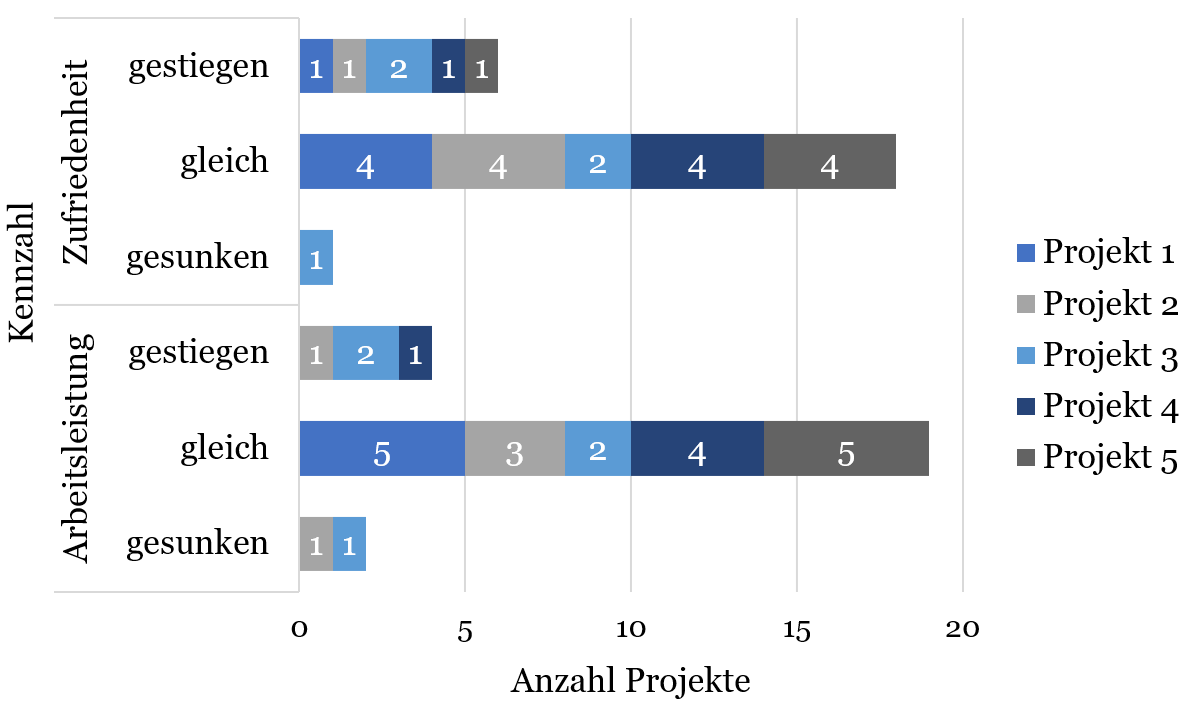
\includegraphics[width=0.9\textwidth]{gfx/verhaeltnis-z-a-projekte.png}
% 	\caption[Veränderung der Zufriedenheit und erwarteten Arbeitsleistung der Mitarbeitenden von unilateralem zu bilateralem Algorithmus nach Projekt]{Veränderung der Zufriedenheit und erwarteten Arbeitsleistung der Mitarbeitenden von unilateralem zu bilateralem Algorithmus nach Projekt}
% 	\label{fig:ergebnisse:abb8}
% \end{figure}

% Aus Abbildung \ref{fig:ergebnisse:abb8} geht hervor, dass in dem Experiment bei einem Großteil der Fälle sowohl hinsichtlich der Auswirkungen auf die Zufriedenheit als auch der zu erwartenden Arbeitsleistung weder eine Verschlechterung noch eine Verbesserung festgestellt werden konnte.
% Weiter ist zu erkennen, dass die Anzahl an Fällen mit Verbesserungen des Anteils unter Einsatz des bilateralen Algorithmus bei beiden Kennzahlen die Anzahl an Fällen mit Verschlechterungen durch Anwendung des bilateralen Algorithmus übersteigt.
% Ein Vergleich der der Veränderungen bei beiden Kennzahlen zeigt darüber hinaus, dass die Zufriedenheit im Verhältnis zu der erwarteten Arbeitsleistung in mehr Fällen gestiegen ist.
% Zugleich führte der bilaterale Algorithmus in zwei Fällen zu einer Verschlechterung der zu erwarteten Arbeitsleistung und in einem Fall zu einer Verschlechterung der Zufriedenheit.
Nachfolgend werden die Auswirkungen auf die Kennzahlen im Detail betrachtet.

\subsection{Auswirkung auf die Zufriedenheit der Mitarbeitenden}
In Abbildung \ref{fig:ergebnisse:abb8} ist der durchschnittliche Anteil an zufriedenen Mitarbeitenden an den unilateralen und an den bilateralen Rankings je Projekt dargestellt.
Der Anteil unter Einsatz des bilateralen Algorithmus ist durch eine blaue Linie dargestellt, während der Anteil unter Anwendung des unilateralen Algorithmus durch eine orangene Linie gekennzeichnet ist.

Abbildung \ref{fig:ergebnisse:abb8} zeigt, dass der Anteil zufriedener Mitarbeitender unter Einsatz des bilateralen Algorithmus bei vier der fünf Projekte im Mittel über dem Anteil unter Anwendung des unilateralen Algorithmus lag.
Lediglich bei Projekt 3 ist zu erkennen, dass die durchschnittlichen Anteile zufriedener Mitarbeitender beider Algorithmen übereinstimmen.
Darüber hinaus ist sichtbar, dass der Anteil zufriedener Mitarbeitender bei Projekt 3 sample-übergreifend bei beiden Algorithmen am niedrigsten und bei Projekt 4 am höchsten lag.
% Diese Struktur stimmt mit der Verteilung der Zufriedenheit der Mitarbeitenden nach Projekt in Abbildung \ref{fig:ergebnisse:abb3} überein.
% Im Mittel wurden demnach in dem Experiment sample-und projektübergreifend durch Einsatz des bilateralen Algorithmus vermehrt Mitarbeitende empfohlen, die eine hohe Zufriedenheit für die jeweiligen Projekte angaben.

\begin{figure}[H]
    \centering
	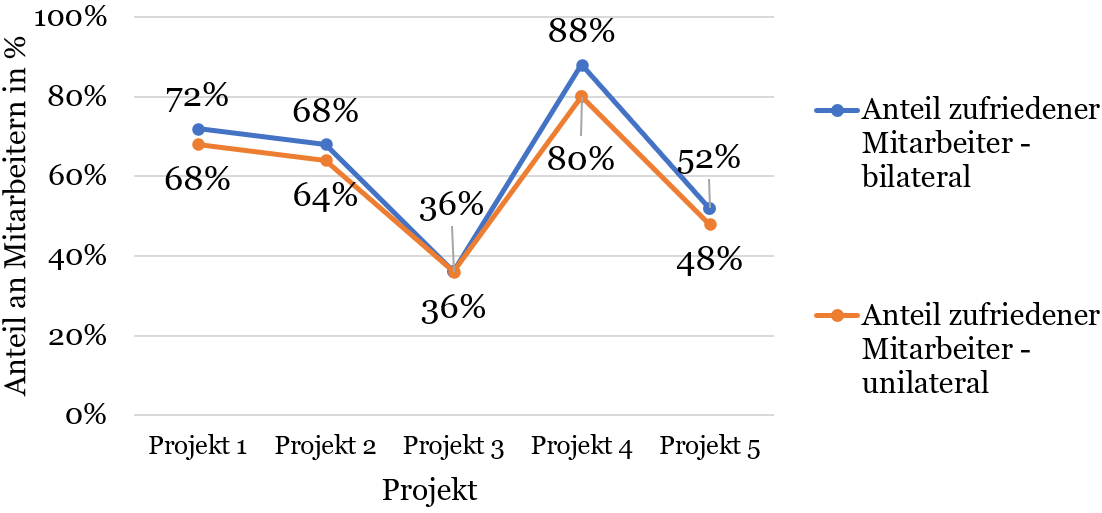
\includegraphics[width=0.95\textwidth]{gfx/verhaeltnis-z-durchschnitt-projekte.png}
	\caption[Anteil zufriedener Mitarbeitender in unilateralen und bilateralen Rankings nach Projekt im Mittel]{Anteil zufriedener Mitarbeitender in unilateralen und bilateralen Rankings nach Projekt im Mittel}
	\label{fig:ergebnisse:abb8}
\end{figure}

Für eine detailliertere Betrachtung der Auswirkung auf die Zufriedenheit ist die Veränderung der Anteile unter Einsatz des unilateralen Algorithmus zu den Anteilen unter Anwendung des bilateralen Algorithmus je Sample und Projekt in Abbildung \ref{fig:ergebnisse:abb9} dargestellt.
Die Abbildung zeigt, bei wie vielen der Projekte der Anteil zufriedener Mitarbeitender durch den bilateralen Algorithmus im Verhältnis zum unilateralen Algorithmus gestiegen, gesunken oder gleich geblieben ist.
Neben der Anzahl an Projekten ist in der Abbildung darüber hinaus abgebildet, in welchem Projekt die jeweilige Änderung erzielt wurde.

\begin{figure}[H]
    \centering
	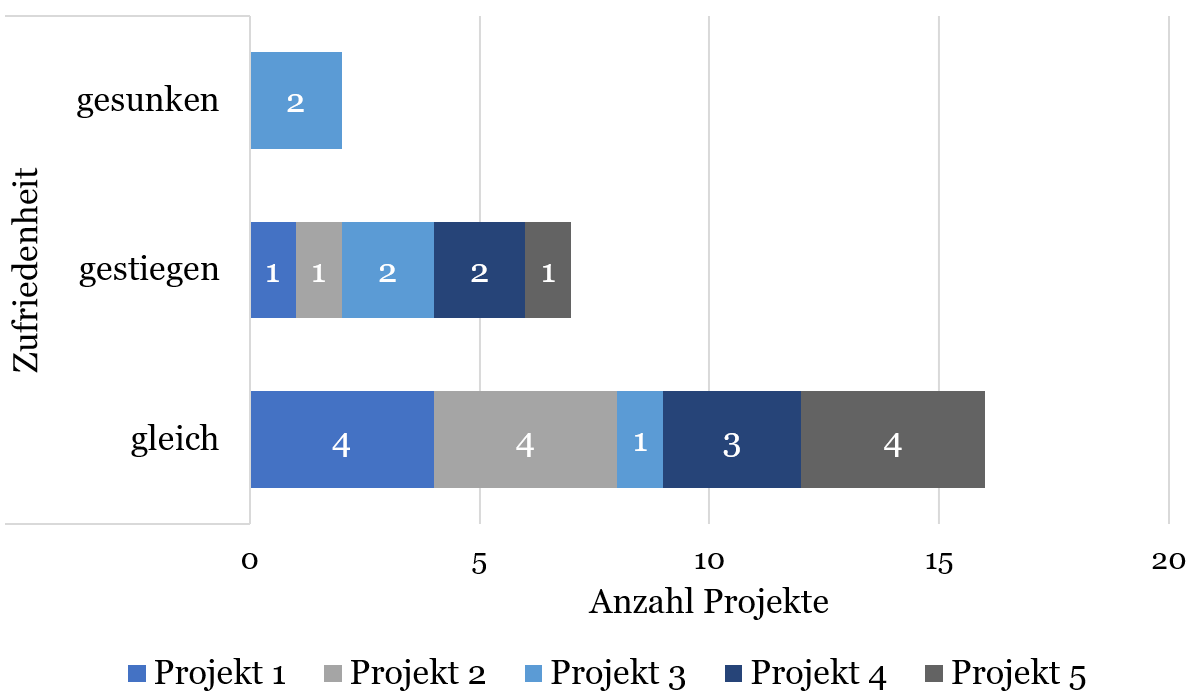
\includegraphics[width=0.95\textwidth]{gfx/verhaeltnis-z-projekte.png}
	\caption[Veränderung der Zufriedenheit der Mitarbeitenden von unilateralem zu bilateralem Algorithmus nach Projekt]{Veränderung der Zufriedenheit der Mitarbeitenden von unilateralem zu bilateralem Algorithmus nach Projekt}
	\label{fig:ergebnisse:abb9}
\end{figure}

Abbildung \ref{fig:ergebnisse:abb9} zeigt, dass in dem Experiment bei 16 der 25 Fälle hinsichtlich der Auswirkungen auf die Zufriedenheit weder eine Verschlechterung noch eine Verbesserung festgestellt werden konnte.
Weiter ist zu erkennen, dass der bilaterale Algorithmus in 28 Prozent der Fällen (7 von 25) für eine höhere Zufriedenheit unter den empfohlenen Mitarbeitenden sorgte.
Lediglich in zwei der 25 Fälle führte der Einsatz des bilateralen Algorithmus zu einer Reduktion des Anteils zufriedener Mitarbeitender im Vergleich zu dem Anteil unter Anwendung des unilateralen Algorithmus.
Aus der Abbildung geht hervor, dass beide Fälle bei Projekt 3 auftraten (hellblauer Balken bei "gesunken").

% Ein Vergleich der der Veränderungen bei beiden Kennzahlen zeigt darüber hinaus, dass die Zufriedenheit im Verhältnis zu der erwarteten Arbeitsleistung in mehr Fällen gestiegen ist.
% Zugleich führte der bilaterale Algorithmus in zwei Fällen zu einer Verschlechterung der zu erwarteten Arbeitsleistung und in einem Fall zu einer Verschlechterung der Zufriedenheit.

\subsection{Auswirkung auf die erwartete Arbeitsleistung der Mitarbeitenden}
Hinsichtlich der zu erwartenden Arbeitsleistung der Mitarbeitenden ist in Abbildung \ref{fig:ergebnisse:abb10} der durchschnittliche Anteil an Mitarbeitenden mit zu erwartend hoher Arbeitsleistung an den unilateralen und an den bilateralen Rankings je Projekt abgebildet.
Wie für die Zufriedenheit in Abbildung \ref{fig:ergebnisse:abb8} ist der Anteil unter Einsatz des bilateralen Algorithmus durch eine blaue und der Anteil unter Anwendung des unilateralen Algorithmus durch eine orangene Linie gekennzeichnet.

\begin{figure}[H]
    \centering
	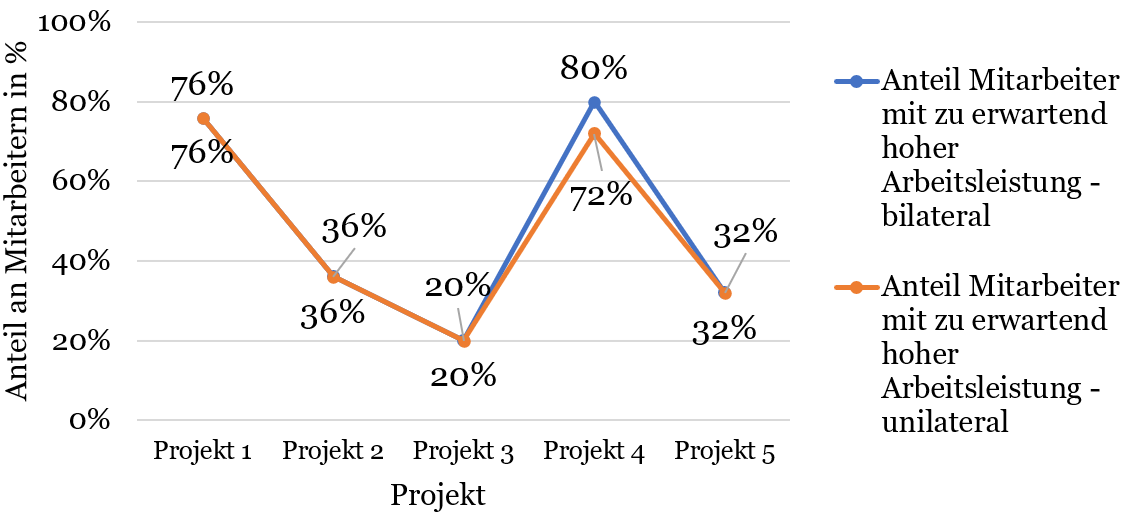
\includegraphics[width=0.95\textwidth]{gfx/verhaeltnis-a-durchschnitt-projekte.png}
	\caption[Anteil an Mitarbeitenden mit zu erwartend hoher Arbeitsleistung in unilateralen und bilateralen Rankings nach Projekt im Mittel]{Anteil an Mitarbeitenden mit zu erwartend hoher Arbeitsleistung in unilateralen und bilateralen Rankings nach Projekt im Mittel}
	\label{fig:ergebnisse:abb10}
\end{figure}

Auffällig ist, dass der durchschnittliche Anteil an Mitarbeitenden mit zu erwartend hoher Arbeitsleistung unter Einsatz des bilateralen Algorithmus bei Projekt 3 und Projekt 4 im Mittel über dem durchschnittlichen Anteil unter Anwendung des unilateralen Algorithmus lag.
Weiter ist zu erkennen, dass der Anteil im Durchschnitt in keinem der Projekte unter Anwendung des bilateralen Algorithmus unter dem durchschnittlichen Anteil unter Einsatz des unilateralen Algorithmus lag.

Ein Vergleich der durchschnittlichen Anteile je Projekt aus Abbildung \ref{fig:ergebnisse:abb10} mit den durchschnittlichen Anteilen zufriedener Mitarbeitender je Projekt in Abbildung \ref{fig:ergebnisse:abb8} zeigt, dass die Kurven einen ähnlichen Verlauf aufweisen.
So ist sowohl der durchschnittliche Anteil zufriedener Mitarbeitender als auch der durchschnittliche Anteil an Mitarbeitenden mit zu erwartend hoher Arbeitsleistung bei Projekt 3 am niedrigsten.
Zugleich ist der durchschnittliche Anteil beider Kennzahlen bei Projekt 4 am höchsten.
Eine Ausnahme davon bildet lediglich der durchschnittliche Anteil an Mitarbeitenden mit zu erwartend hoher Arbeitsleistung unter Einsatz des unilateralen Algorithmus.
Dessen Höhepunkt liegt bei Projekt 1.

Abbildung \ref{fig:ergebnisse:abb11} stellt die Veränderung der Anteile an Mitarbeitenden mit zu erwartend hoher Arbeitsleistung unter Einsatz des unilateralen Algorithmus zu den Anteilen unter Anwendung des bilateralen Algorithmus je Sample und Projekt dar.

\begin{figure}[H]
    \centering
	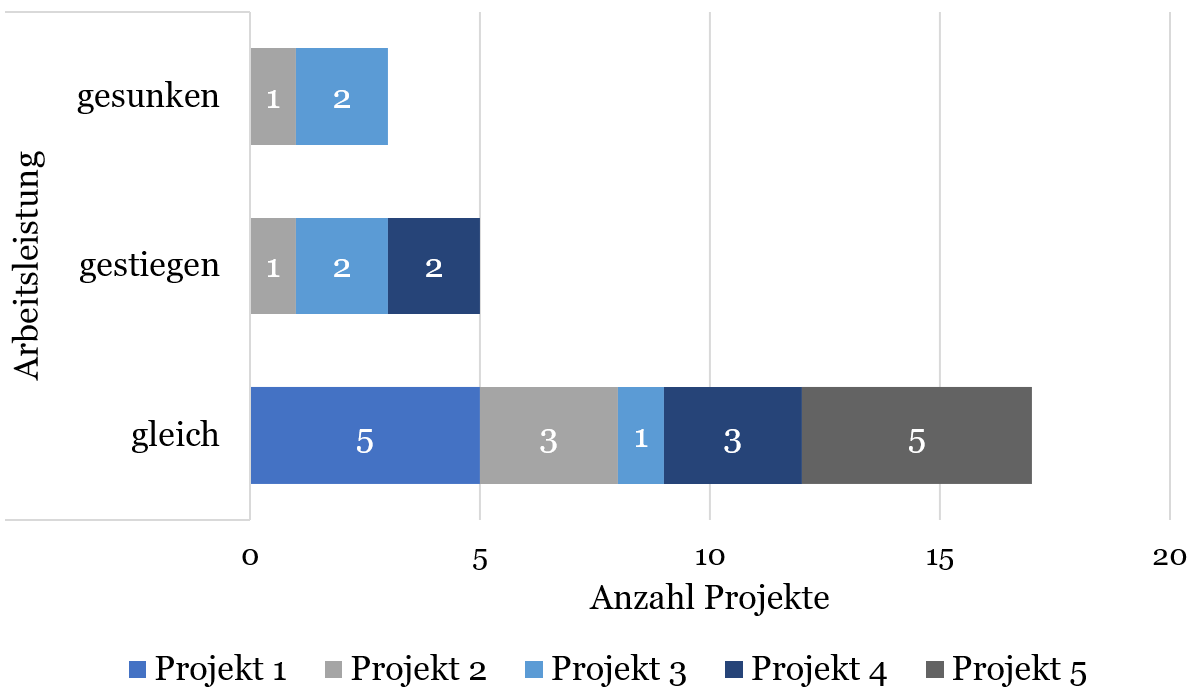
\includegraphics[width=0.95\textwidth]{gfx/verhaeltnis-a-projekte.png}
	\caption[Veränderung der erwarteten Arbeitsleistung der Mitarbeitenden durch die Manager von unilateralem zu bilateralem Algorithmus nach Projekt]{Veränderung der erwarteten Arbeitsleistung der Mitarbeitenden durch die Manager von unilateralem zu bilateralem Algorithmus nach Projekt}
	\label{fig:ergebnisse:abb11}
\end{figure}

Daraus geht hervor, dass in dem Experiment bei 17 der 25 Fälle hinsichtlich der Auswirkungen auf die erwartete Arbeitsleistung weder eine Verschlechterung noch eine Verbesserung festgestellt wurde.
Die Abbildung zeigt, dass sowohl Projekt 1 als auch Projekt 5 sample-übergreifend überhaupt keine Veränderung aufwiesen (blauer und grauer Balken bei "gleich").
Weiter ist zu erkennen, dass der bilaterale Algorithmus in 5 der 25 Fälle sogar zu einer höheren zu erwartenden Arbeitsleistung der empfohlenen Mitarbeitenden führte. 
In drei der 25 Fälle führte der Einsatz des bilateralen Algorithmus zu einer Reduktion des Anteils an Mitarbeitenden mit zu erwartend hoher Arbeitsleistung im Vergleich zu dem Anteil unter Anwendung des unilateralen Algorithmus.
Aus der Abbildung geht hervor, dass diese Fälle bei Projekt 2 und Projekt 3 auftraten (hellgrauer und -blauer Balken bei "gesunken").

\subsection{Einfluss der Gewichtung von Fähigkeiten und Präferenzen}
Neben den Auswirkungen des bilateralen und unilateralen Algorithmus wurde darüber hinaus der Einfluss der Gewichtung von Fähigkeiten und Präferenzen auf Zufriedenheit und Arbeitsleistung betrachtet.
Tabelle \ref{tab:ergebnisse:tab1} zeigt je Sample, welcher $\alpha$-Wert als optimales Gewicht der Fähigkeiten ermittelt wurde.

\begin{table}[htbp]
    \begin{center}
    \begin{tabular}{c|c}
    {\textbf{Sample}} & {\boldmath$\alpha$}\\
    \hline
    0 & 0.7868 \\
    \hline
	1 & 0.6068 \\
    \hline
    2 & 0.6823 \\
    \hline
	3 & 0.7805 \\
    \hline
	4 & 0.6681 \\
    \end{tabular}
    \end{center}
    \caption[Ermitteltes Gewicht $\alpha$ je Sample]{Ermitteltes Gewicht $\alpha$ je Sample}
	\label{tab:ergebnisse:tab1}
\end{table}

Daran ist zu erkennen, dass die ermittelten Gewichte anhand unterschiedlicher Kombinationen der Trainingsdatensätze alle in einen Bereich zwischen 0.6 und 0.8 fielen.
Die Veränderung des Anteils an zufriedenen Mitarbeitenden von unilateralem zu bilateralem Algorithmus in Abhängigkeit des Gewichts $\alpha$ ist in Abbildung \ref{fig:ergebnisse:abb12} dargestellt.
Darin ist abgebildet, bei wie vielen Projekten der Anteil an zufriedenen Mitarbeitenden im Vergleich zum unilateralen Algorithmus gestiegen, gesunken oder gleich geblieben ist.

\begin{figure}[H]
    \centering
	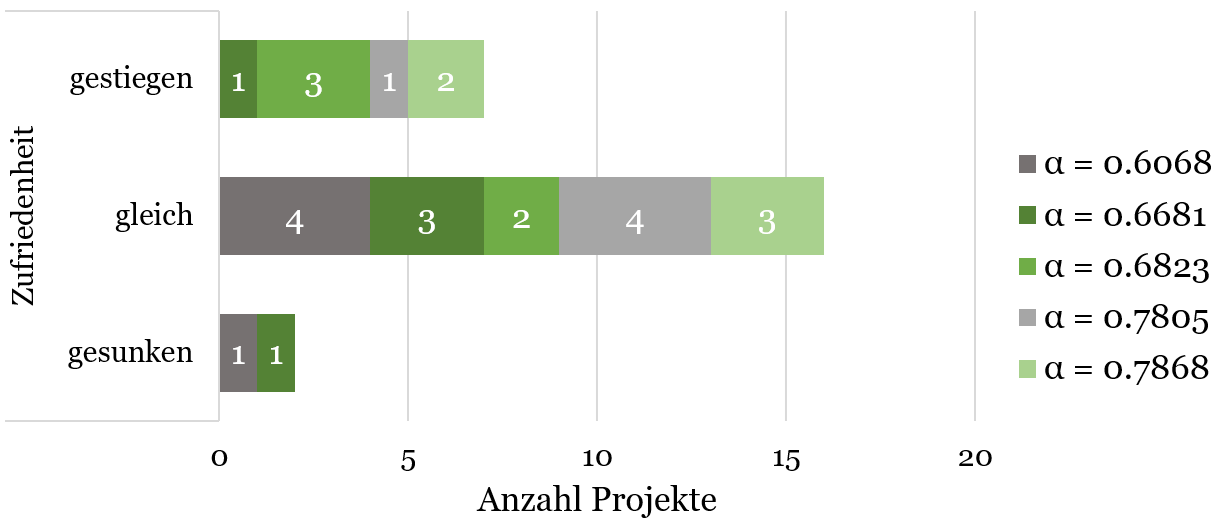
\includegraphics[width=0.95\textwidth]{gfx/verhaeltnis-z-nach-alpha-ges.png}
	\caption[Veränderung der Zufriedenheit der Mitarbeitenden von unilateralem zu bilateralem Algorithmus nach $\alpha$-Wert]{Veränderung der Zufriedenheit der Mitarbeitenden von unilateralem zu bilateralem Algorithmus nach $\alpha$-Wert}
	\label{fig:ergebnisse:abb12}
\end{figure}

Abbildung \ref{fig:ergebnisse:abb12} zeigt, dass für keines der Gewichte alle fünf Projekte einer Kategorie ("gestiegen", "gleich", "gesunken") zugeordnet wurden.
Insgesamt ist zu erkennen, dass mit Ausnahme des $\alpha$-Werts von 0.6068 (Sample 1) mit jedem Gewicht in mindestens einem der fünf Projekte eine Steigerung der Zufriedenheit erreicht werden konnte.
Auffällig ist außerdem, dass die zwei Fälle mit gesunkener Zufriedenheit in den Samples mit den niedrigsten Gewichten für $\alpha$ und demnach den höchsten Gewichten für die Präferenzen erzielt wurden.
Die meisten Projekte mit gestiegener Zufiedenheit bei den empfohlenen Mitarbeitenden konnten mit dem Gewicht 0.6823 (Sample 2, 3 Projekte) erzielt werden (grüner Balken bei "gestiegen").

Hinsichtlich des Einflusses auf die zu erwartende Arbeitsleistung der Mitarbeitenden ist in Abbildung \ref{fig:ergebnisse:abb13} die Veränderung des Anteils an Mitarbeitenden mit zu erwartend hoher Arbeitsleistung von unilateralem zu bilateralem Algorithmus in Abhängigkeit des Gewichts $\alpha$ abgebildet.

\begin{figure}[H]
    \centering
	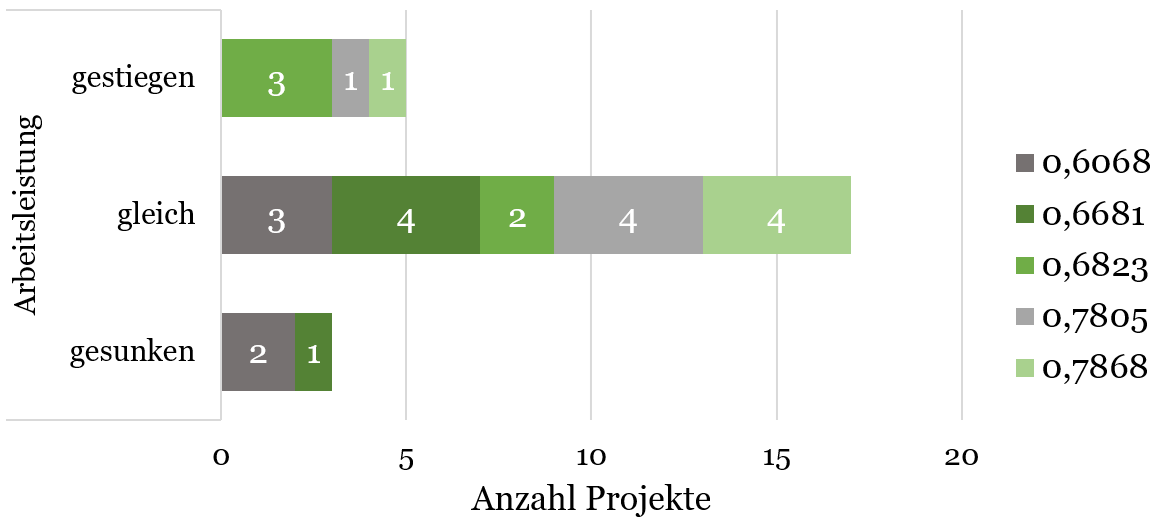
\includegraphics[width=0.95\textwidth]{gfx/verhaeltnis-a-nach-alpha-ges.png}
	\caption[Veränderung der zu erwartenden Arbeitsleistung der Mitarbeitenden von unilateralem zu bilateralem Algorithmus nach $\alpha$-Wert]{Veränderung der zu erwartenden Arbeitsleistung der Mitarbeitenden von unilateralem zu bilateralem Algorithmus nach $\alpha$-Wert}
	\label{fig:ergebnisse:abb13}
\end{figure}

Analog zu der Zufriedenheit ist in Abbildung \ref{fig:ergebnisse:abb13} zu erkennen, dass bei keinem der Gewichte alle fünf Projekte einer Kategorie zugeordnet wurden.
Weiter geht aus der Abbildung hervor, dass die drei Projekte mit gesunkener Arbeitsleistung durch die Samples mit den niedrigsten Gewichten für die Fähigkeit bewirkt wurden (2 Projekte mit $\alpha$=0.6068, 1 Projekt mit $\alpha$=0.6681).
Wie für die Zufriedenheit konnte eine Steigerung der Arbeitsleistung bei den meisten Projekten mit dem Gewicht 0.6823 (Sample 2, 3 Projekte) erreicht werden (Vgl. Abbildung \ref{fig:ergebnisse:abb12}).
Mit dem höchsten Gewicht unter den Samples (Sample 4, $\alpha$=0.7868) konnte die Zufriedenheit lediglich in einem Projekt gesteigert werden (hellgrüner Balken bei "gestiegen").
% GRAPHEN ANPASSEN!


\shorthandon{"}